\documentclass{../../templates/amendment}
\usepackage{blindtext}
\usepackage[ngerman]{babel}
\usepackage{graphicx}
\usepackage{subcaption}
\usepackage[skip=2pt,font=small]{caption}

% \usepackage{showframe}
\occasion[Berzirksvertretung]{Bezirksvertretung Innenstadt-West}
\date{29. Dezember 2024}
\setcounter{nthantrag}{1}
\begin{document}

\begin{boxed}{Sportanlage Am Tremonipark / Haldenstr.}{Jan Lucas Brause, Maximilian Sackel}
    Die neue Calisthenicsanlage im Tremoniapark bildet in Kombination mit dem Basket- und Fußballplatz einen Treffpunkt für alle Generationen und den Querschnitt der Bevölkerung.
    Neben spielenden Kindern auf dem Bolzplatz und Jugendlichen auf dem Basketballplatz finden sich dort genauso Erwachsene, die ihre Zeit am Calisthenics Park zum Trainieren nutzen.
    Ebenso wird die Sportanlage von vielen Studierenden und jungen Berufstätigen als unverbindliche und kostenlose Trainingsmöglichkeit äußerst gut angenommen.
    Zudem haben sich bereits Sportvereine gebildet, welche diese Sportanlage für
    ihren Trainingsmittelpunkt nutzen und somit das angeleitete Sportangebot und
    die sozialen Strukturen vor Ort stärken.

    Die Nutzung der Sportanlagen ist in den Wintermonaten in den Nachmittags und
    Abendstunden nicht möglich, da bei frühem Einbruch der Dunkelheit die
    Anlage komplett finster ist, da jegliche Beleuchtung fehlt.
    Dies führt dazu, dass die Sportanlage weitestgehend von Sportlern und
    spielenden ungenutzt bleibt und zu einem Angstraum wird.
    Das Koten von nicht angeleinten Hunden, Schreckschusswaffen gebrauch,
    Drogendelikte oder Wohnungslose sind im Schutz der Dunkelheit dort nicht
    selten anzutreffen.
    Vandalismus an den Sportstätten kann durch die Installation von Beleuchtung
    und der damit einhergehenden längeren Nutzung vorgebeugt werden.
    Das umgliegende dichte Unterholz wird regelmäßig von Personen welche
    Abseits der Wege gehen aufgesucht.
    Tauchen diese aufeinmal in der Dunkelheit aus dem Gebüschen auf sorgt dies
    regelmäßig für große Schockmomente, wodurch der Standort für besonders
    Schutzbedürftige nicht attraktiv ist.

    Eine Beleuchtung mit Zeitschaltbetrieb bis beispielsweise 21:00~Uhr
    verlängert die Nutzungsdauer und sorgt durch die Anwesenheit von
    Trainierenden und Sportlern dafür, dass die Fläche unattraktiver für
    benannte dubiose Tätigkeiten wird.
    Des Weiteren wird durch eine Beleuchtung in den Abendstunden ein
    ausgeweitetes Sportangebot für zeitlich und finanziell eingeschränkte Bürger
    und Bürgerinnen geschaffen.

    Die Lichtverschmutzung lässt sich durch eine Zeitschaltung auf die
    Nutzungsdauer minimieren.
    Ein besonders grosses Tierreich welches von dem Licht gestört werden
    könnte ist aufgrund der Menschen und Hunde welche regelmäßig das Unterholz
    durchkemmen nicht zu erwarten.
    % Bei der Vielzahl an nicht angeleiten Hunden die regelmäßig das Gebiet dort
    % durchkemmen ist nicht davon auszugehen, dass sich dort ein
    % Eine Lichtverschmutzung besteht nicht, da es sich um urbanes Gebiet handelt und einige Hundehalter ihre Tiere ohne Leine laufen lassen.
    Störung der Anwohner aufgrund der Beleuchtung können aufgrund der Entfernung
    ausgeschlossen werden.
    Bei einer ähnlichen Spiel- und Sportanlage an der Düsterstraße in Körne
    wurde bereits eine Beleuchtung ohne das Verlegen von Stromleitungen im
    Erdreich mittels einer integrierten Solareinheit realisiert und wäre auch
    hier wünschenswert.

    Zudem möge die Bezirksvertretung beschließen im Sinne der beschlossenen
    Richtlinie (EU) 2020/2184 des Europäischen Parlaments und des Rates vom 16.
    Dezember 2020 über die Qualität von Wasser für den menschlichen Gebrauch
    (ABl. L 435 vom 23.12.2020, S. 1) zur Bereitstellung von kostenlosem
    Trinkwasser im öffentlichen Raum einen Trinkwasserbrunnen in direkter Nähe
    zu den Sportstätten aufzustellen.
    Der Gesetzentwurf setzt die Regelung nach Artikel 16 Absatz 2 Satz 1 der
    Richtlinie um, wonach die Mitgliedstaaten sicherstellen, dass Leitungswasser
    zur Nutzung als Trinkwasser an öffentlichen Orten durch Innen- und Außenanlagen
    bereitgestellt wird, soweit dies technisch durchführbar und unter
    Berücksichtigung des Bedarfs und der örtlichen Gegebenheiten, wie Klima und
    Geografie, verhältnismäßig ist (Paragraf 50 Absatz 1 Satz 2 WHG neu).

    Im Anhang sind Abbildungen für eine bessere Einsicht der Sachlage angefügt.
    Einen Ortstermin zu einer Machbarkeitsstudie, sowie die Bündelung weiterer möglicher Verbesserung und Sanierungsvorschläge, halten wir für sinnvoll.

    Über eine Bearbeitung und positive Rückmeldung würden wir uns sehr freuen.
    Selbstverständlich stehen wir gerne für Rückfragen und zur Terminvereinbarung zur Verfügung.

    \begin{figure}[htpb]
        \centering
        \begin{subfigure}[]{0.3\textwidth}
            \begin{center}
                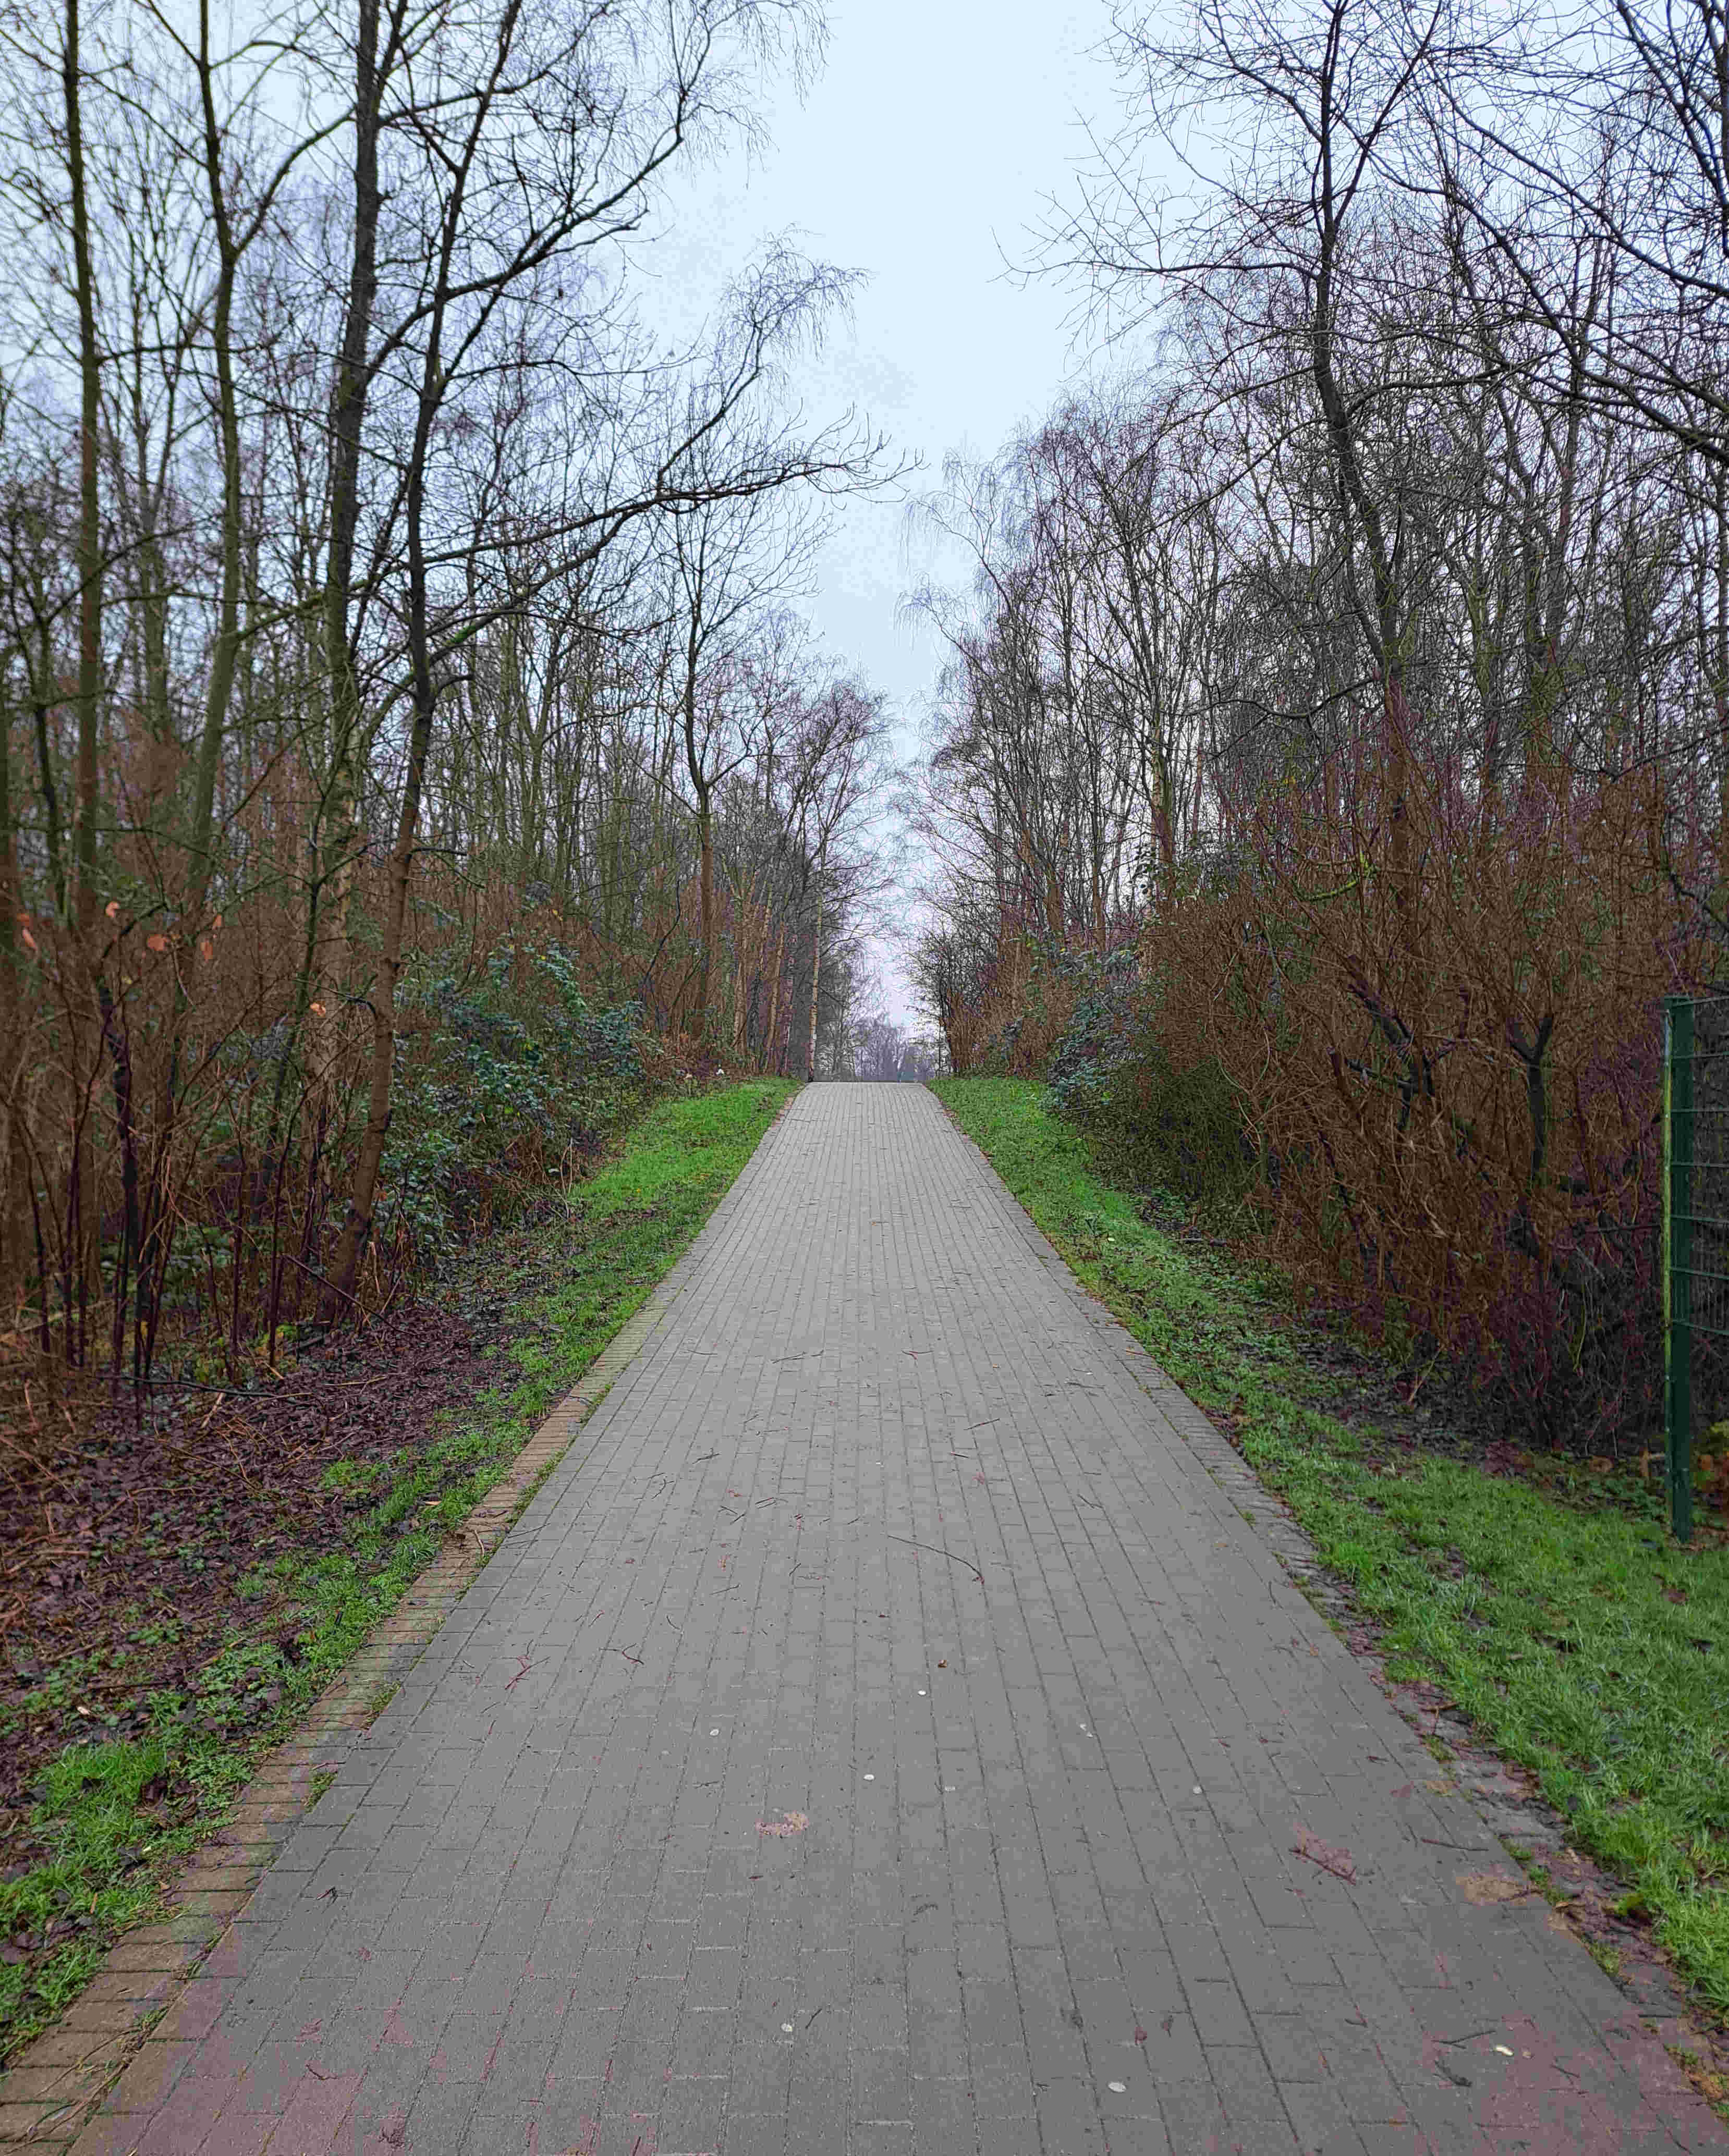
\includegraphics[width=\linewidth]{pictures/photo1.jpg}
                \caption{Dicht bewachsener Ziehweg der passiert
                werden muss um zu den Sportanlagen zu gelangen.}%
            \end{center}
        \end{subfigure}
        \begin{subfigure}{0.5\textwidth}
            \begin{center}
                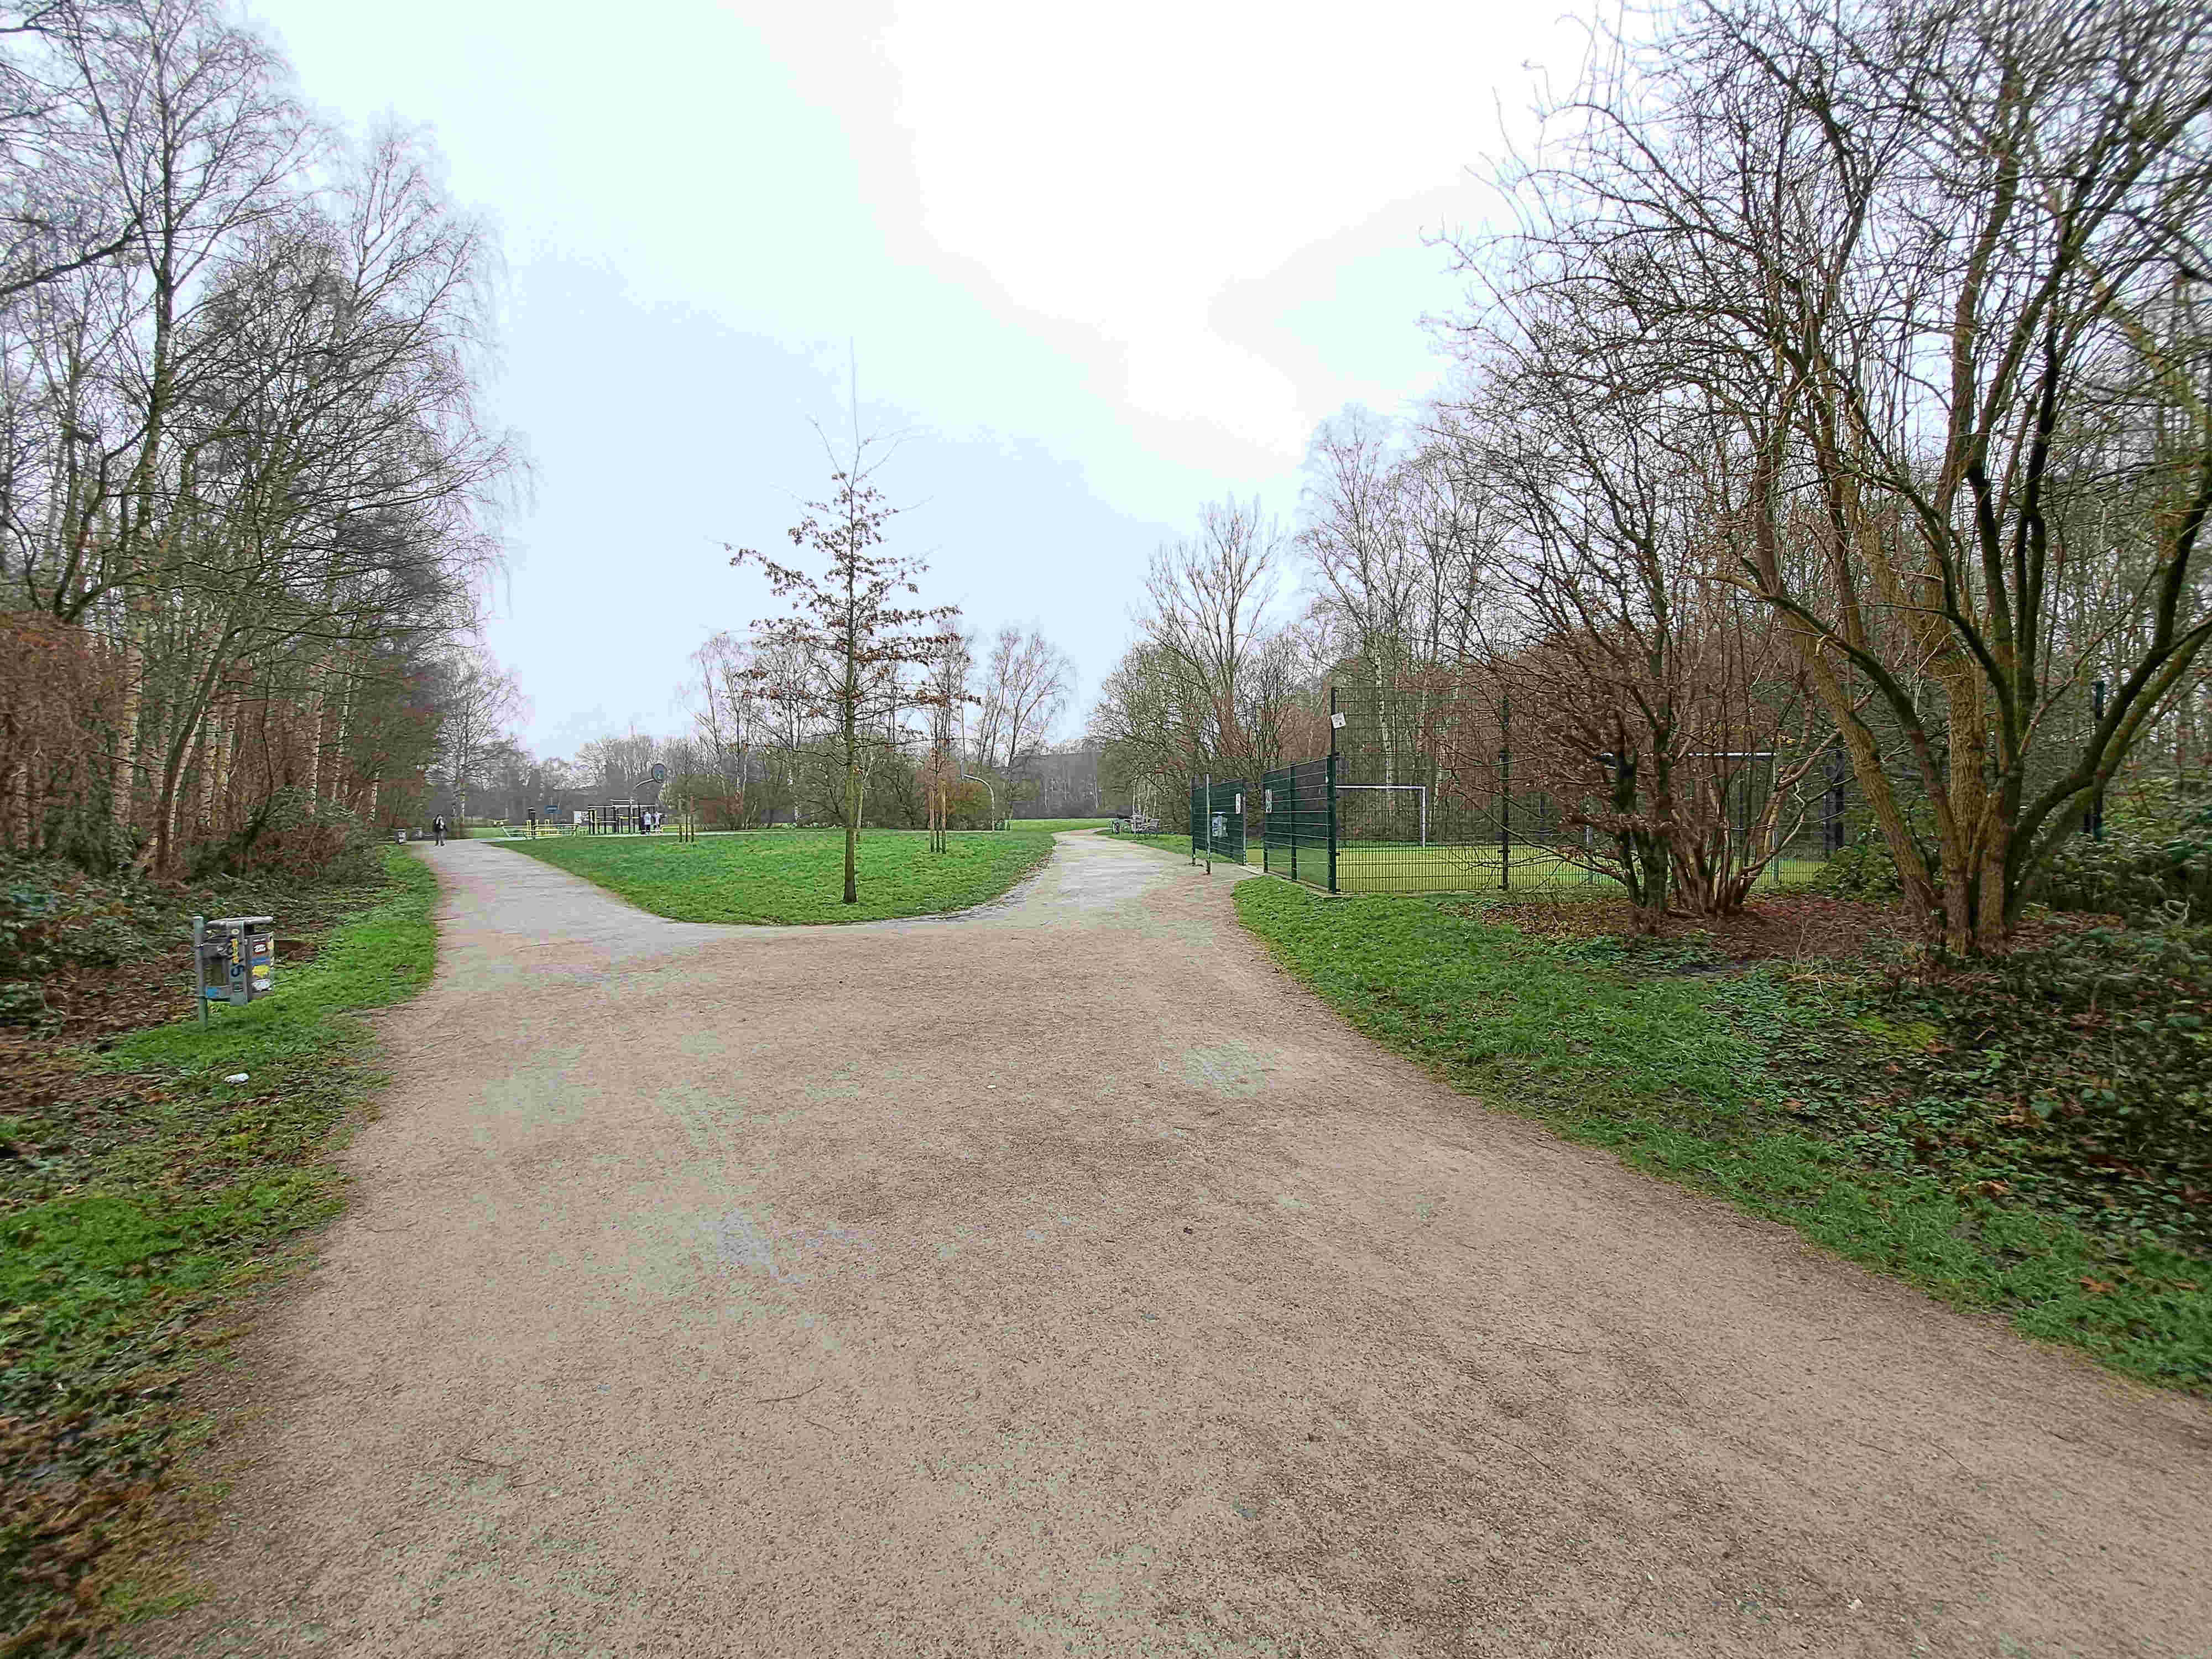
\includegraphics[width=\linewidth]{pictures/photo5.jpg}
                \caption{Übersicht der räumlichen Gegebenheiten. Rechts der
                    Fussballplatz, in der Mitte der Basketballplatz und hinten links
                die Calisthenics-Anlage.}%
            \end{center}
        \end{subfigure}
        \caption{Die gesamte Anlage ist von dichten Unterholz umgeben. Der Charm
            des Trainings im Grünen in den Sommermonaten,
            schirmt im Winter jegliches Streulicht von benachbarten Gebäden ab,
            sodass die gesamte Anlage finster und unbrauchbar in den Abendstuden der Wintermonate wird.
        }
    \end{figure}

    \begin{figure}[htpb]
        \centering
        \begin{subfigure}[]{0.32\textwidth}
            \begin{center}
                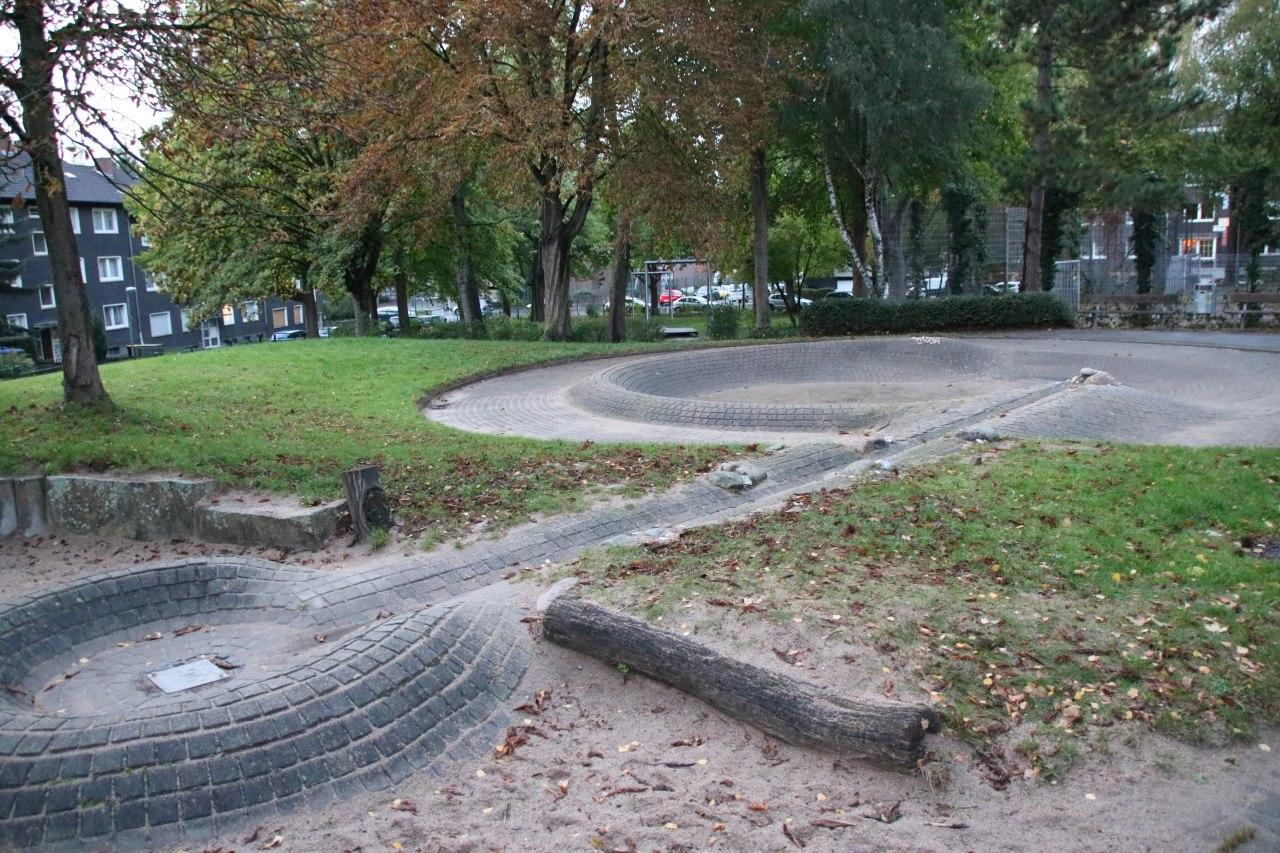
\includegraphics[width=\linewidth]{pictures/photo2.jpg}
                \caption{Basketballplatz}%
            \end{center}
        \end{subfigure}
        \begin{subfigure}[]{0.32\textwidth}
            \begin{center}
                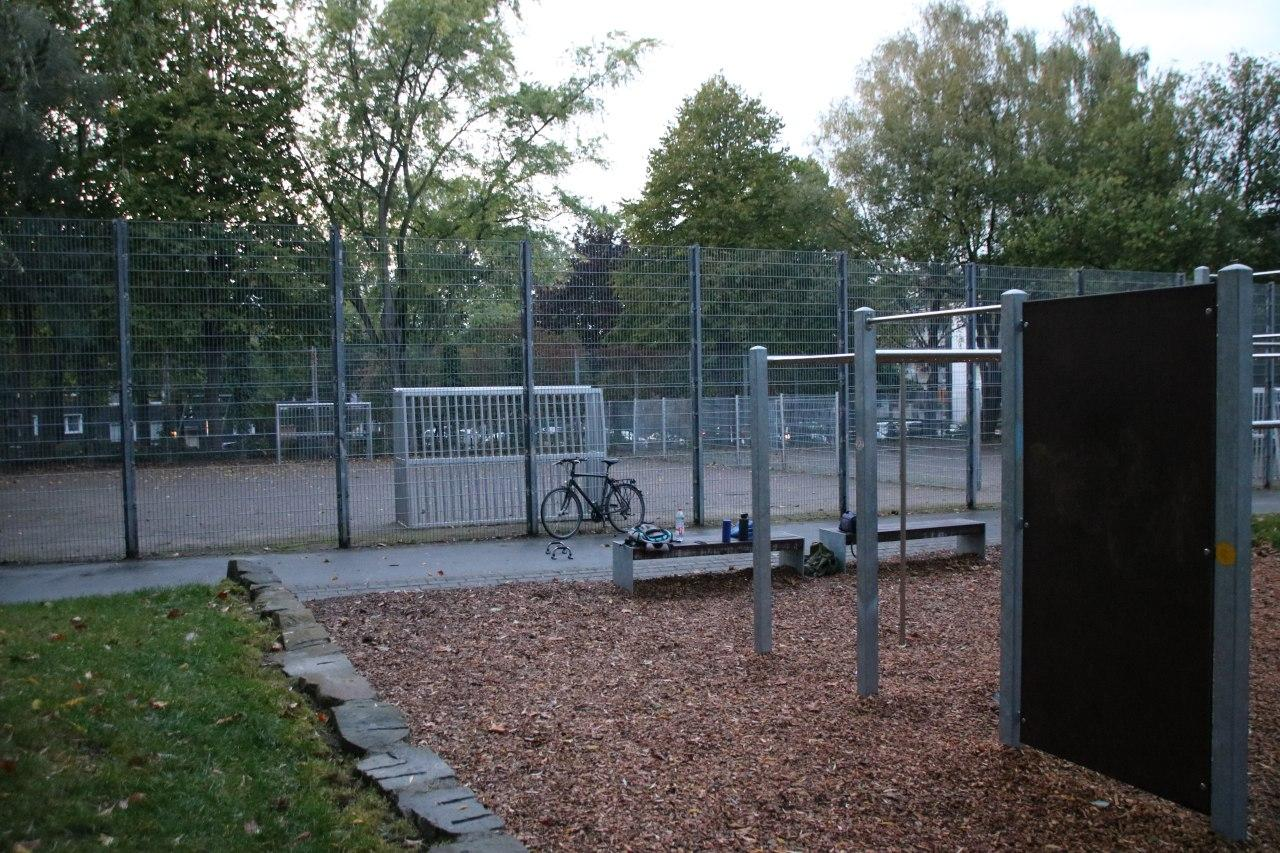
\includegraphics[width=\linewidth]{pictures/photo3.jpg}
                \caption{Calisthenics-Anlage}%
            \end{center}
        \end{subfigure}
        \begin{subfigure}[]{0.32\textwidth}
            \begin{center}
                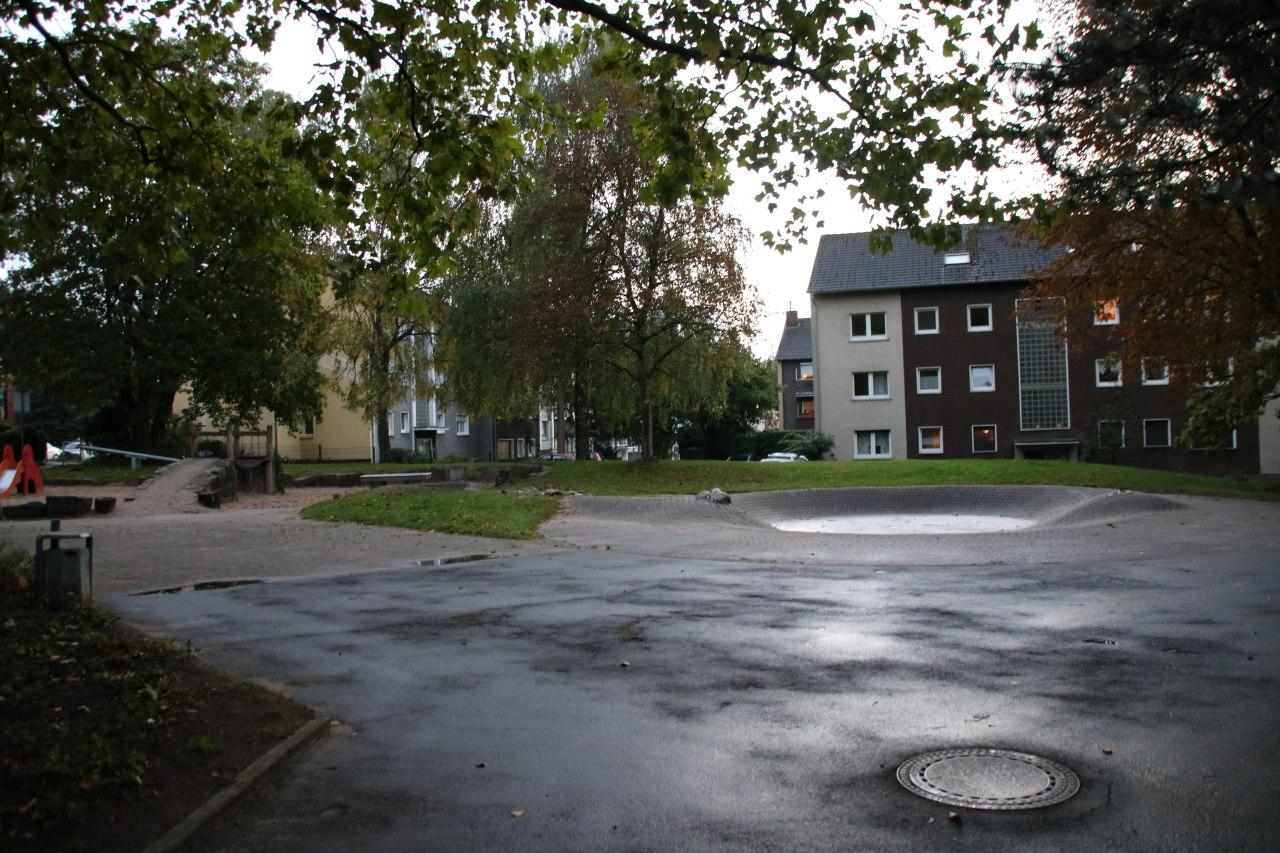
\includegraphics[width=\linewidth]{pictures/photo4.jpg}
                \caption{Fussballplatz}%
            \end{center}
        \end{subfigure}
        \caption{Sportstätten die in den Wintermonaten in den Abendstunden aufgrund der fehlenden
            Beleuchtung nicht mehr genutzt werden koennen und einen Angstraum
        bilden, sobald keine aktiven Sportler mehr da sind.}
    \end{figure}

    \begin{figure}[htpb]
        \centering
        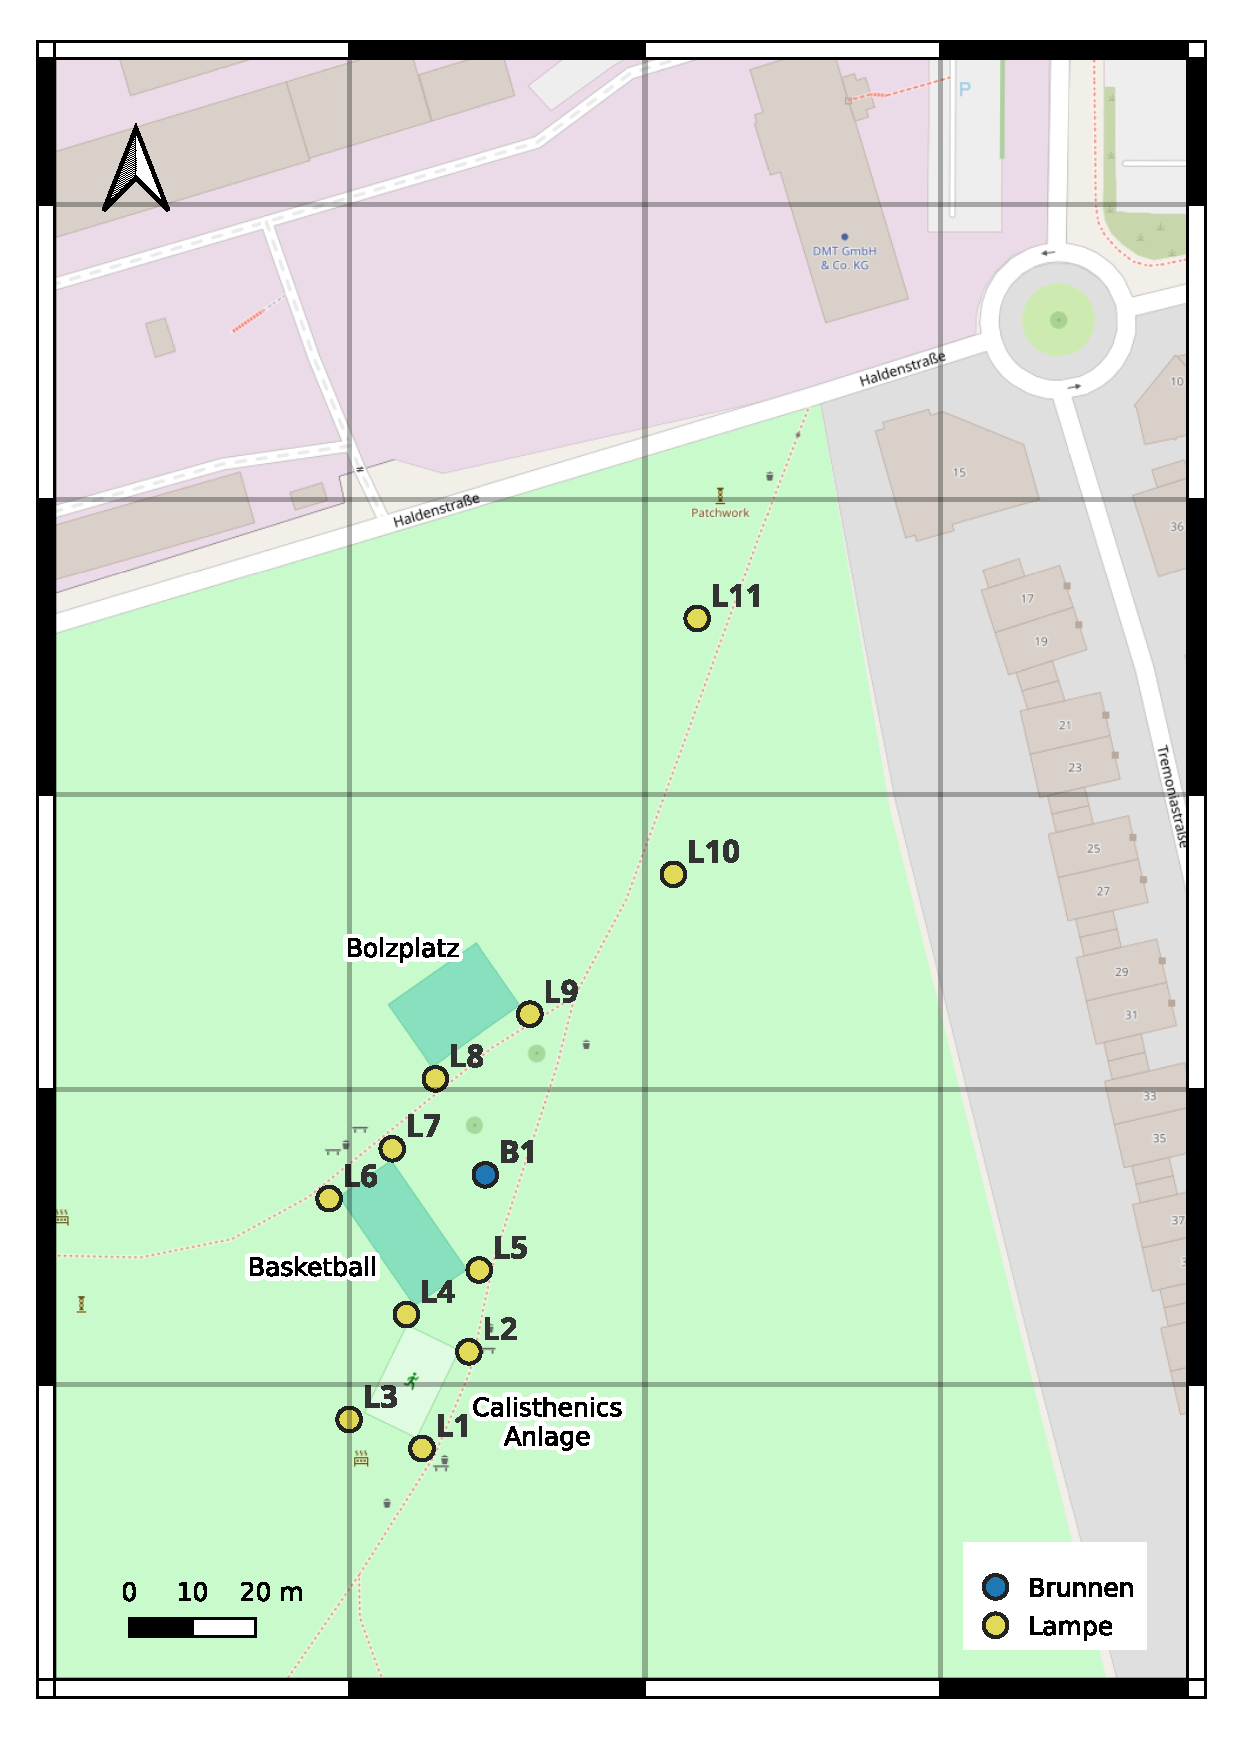
\includegraphics[width=0.8\linewidth]{pictures/map3.pdf}
        \caption{Übersicht zur räumlichen Situation der unbeleuchteten Fläche
            mit Vorschlägen für geeignete Standorten von Lampen \textbf{L1} bis
        \textbf{L11} sowie eines Trinkwasserspenders \textbf{B1}.}%
        \label{fig:}
    \end{figure}
\end{boxed}

\end{document}
